\documentclass[12pt, conference]{IEEEtran}
% \IEEEoverridecommandlockouts
% The preceding line is only needed to identify funding in the first footnote. If that is unneeded, please comment it out.



\usepackage{cite}
\usepackage{amsmath,amssymb,amsfonts}
\usepackage{algorithmic}
\usepackage{graphicx}
\usepackage{textcomp}
\usepackage{xcolor}
\usepackage{hyperref}
\usepackage{wrapfig}
\def\BibTeX{{\rm B\kern-.05em{\sc i\kern-.025em b}\kern-.08em
    T\kern-.1667em\lower.7ex\hbox{E}\kern-.125emX}}
    
% for image assets    
\graphicspath{ {./images/} }

\begin{document}

\title{Natural Language Inference Using Various Types of Neural Networks}

\author{\IEEEauthorblockN{Nukit Tailor}
\IEEEauthorblockA{\textit{IIIT, Hyderabad} \\
2020114012 \\
nukit.t@research.iiit.ac.in}
\and
\IEEEauthorblockN{George Paul}
\IEEEauthorblockA{\textit{IIIT, Hyderabad} \\
2021121006 \\
george.paul@research.iiit.ac.in}
\and
\IEEEauthorblockN{Amal Sunny}
\IEEEauthorblockA{\textit{IIIT, Hyderabad} \\
2021121011 \\
amal.sunny@research.iiit.ac.in}
}

\maketitle

\section{Introduction}
Natural Language Inference is a Natural Language Processing task in which, given a premise ($P$) and a hypothesis $(H)$, we find out whether the hypothesis can be deduced from the premise. i.e.\\
$$
P \implies H
$$
For this task we employ the power of neural networks of various types and architectures to create neural models that can predict whether a $(P, H)$ pair is an entailment (E), contradiction (C) or cannot be determined and is neutral (N).\\
Essentially our task is to create a three-label classifier for these $(P, H)$ pairs.\\

\section{Applications}

\subsection{Paraphrasing}
The task of paraphrasing a text in different words is dependent on knowing whether the sentences that are paraphrased can be inferred from the original sentences. And not only inferred, information-wise, the text must be equivalent to the paraphrasing.

\subsection{Summarising}
Similar to paraphrasing, when the summary of a text can be inferred from the original text, it can be considered a faithful summary. As well as checking whether all the important parts of the text can be inferred from the summary. 

\section{Related Literature}

\subsection{A large annotated corpus for learning natural language inference}
Bowman addresses the lack of large datasets for the NLI task in this paper \cite{b1}. The team at Stanford employ crowdsourcing techniques to gather a large 570 thousand strong dataset meant to train machine learning models.

\subsection{Lessons from Natural Language Inference in the Clinical Domain}
This paper\cite{b2} introduces the MedNLI dataset and explores the usability of neural networks for Natural Language Inference.

\subsection{A Broad-Coverage Challenge Corpus for
Sentence Understanding through Inference}
Bowman's paper \cite{b3} expands on the SNLI dataset, uses the same format and adds upto 430 thousand pairs for the training of neural networks with the introduction of the MultiNLI dataset.

\subsection{GloVe: Global Vectors for Word Representation}
GloVe is a set of pre-trained word embeddings that are of high quality, that were introduced in this 2014 paper\cite{b4}. GloVe is indispensible when encoding text from datasets into a weight vector that conveys its meaning.

\section{Datasets Used}

\subsection{SNLI}
Introduced with \cite{b1}, SNLI consists of 570 thousand pairs of premises and hypotheses. The dataset was collected using Amazon Mechanical Turk which employs turk workers and asks them to annotate pairs of sentences with either Contradiction (C), Entailment (E) or Neutral (N). Each pair was annotated by exactly five different turk workers and if a consensus was reached by at least three of the workers then a "gold label" was assigned to the premise-hypothesis pair which will be the same as the consensus.

\subsection{MultiNLI}
The Multi-Genre Natural Language Inference (MultiNLI) corpus was introduced with \cite{b3} and follows a similar format to the SNLI dataset with 5 attempts at labelling by crowdsourced workers. Those pairs with a consensus are also labelled as such. It can be considered as an extension to the 570 thousand pairs of SNLI. The main difference being that the texts are taken from a wider variety of contexts and genres and from both spoken and written text.  

\section{Approaches}
Initially, an approach using the hand-built features of the data and rule-based approaches was considered. Aspects such as edit distances and word overlap were looked into. The approach was scrapped due to a lack of true understanding in these matters.\\
The second broad approach, as suggested by the related literature, was to create a neural model. On further reading and investigation, many improvements could be made to the default neural network to improve its accuracy for the NLI task:

\subsection{Simple RNN with ReLU}
Context being an important part of the classifying process, our first approach involved the use of a Recurrent Neural Network. RNNs maintain a sort of "memory" and context along the run time of the network by utilising output connections that feed directly back into the input of the same node. 
$$
h_t = f(h_{t-1}, x_t)
$$
Where $x_t$ is the input at time $t$ and $h_t$ is the state of a node at time $t$. \\
This RNN model was run with neurons that applied the Rectified Linear Unit (ReLU) activation function (Fig.1):
$$
\text{ReLU}(x)=\max(0,x)
$$
\begin{figure}[h]
\centering
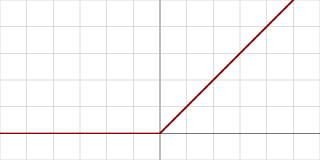
\includegraphics[width=6cm]{images/relu.png}
\caption{Plot of the ReLU Activation Function}
\end{figure}

% \textbf{Accuracy Results:}
% \begin{itemize}
%     \item{When trained and tested on SNLI: $81.74$\%}
%     \item{When trained and tested on MultiNLI: $68.28$\%}
% \end{itemize}

\subsection{Simple RNN with Sigmoid}
Using a similar Recurrent Neural Network but this time the neurons that use the sigmoid function (Fig.2) for activation purposes:
$$
S(x)=\frac {e^{x}}{e^{x}+1}=1-S(-x)
$$
\begin{figure}[h]
\centering
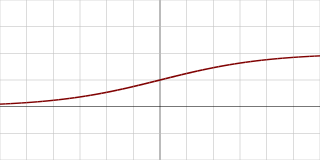
\includegraphics[width=6cm]{images/sigmoid.png}
\caption{Plot of the Sigmoid Activation Function}
\end{figure}

% \textbf{Accuracy Results:}
% \begin{itemize}
%     \item{When trained and tested on SNLI: $81.65$\%}
%     \item{When trained and tested on MultiNLI: $67.84$\%}
% \end{itemize}

\subsection{Simple RNN with Softmax}
RNNs proved to be effective and thus we attempted one more modification to the model by using the softmax function for activation of the neurons:
$$
\sigma (z) = \frac{e^{x_{i}}}{\sum_{j=1}^{K}e^{x_{j}}}
$$
for $ i = 1,...,K$\\

% \textbf{Accuracy Results:}
% \begin{itemize}
%     \item{When trained and tested on SNLI: $79.69$\%}
%     \item{When trained and tested on MultiNLI: $67.10$\%}
% \end{itemize}

\subsection{LSTM Model}

LSTM (Long Short-Term Memory) Neural Networks were our next approach. The advantages that LSTMs have over RNNs are many. \\
\begin{figure}[h]
\centering
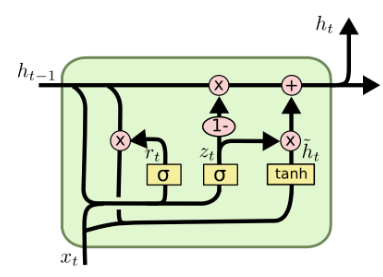
\includegraphics[width=6cm]{images/lstm.png}
\caption{A representational diagram of an LSTM cell}
\end{figure}
LSTMs have an input gate, forget gate and an output gate (Fig.3). A core idea in the architecture of LSTMs is the constantly maintained cell state that allows a maintenance of context and not only remembering past information but also learning new information quickly as a merit of the forget gate. \\ 
As a result of this we should get a model that understands the context of its inputs faster and thus trains in a way that takes context into account more accurately.\\
LSTMs are not without their demerits though. Due to the increased amount of computation per cell, training times are much higher for LSTM models.

\subsection{GRU Model}
The Gated Recurrent Unit (GRU) model combines the input and forget gate into a single update gate as well as merging the cell and hidden states. This leads to an overall simpler architecture.
\begin{figure}[h]
\centering
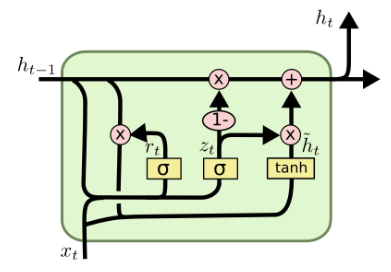
\includegraphics[width=6cm]{images/gru.png}
\caption{A representational diagram of a GRU cell}
\end{figure}

\subsection{BERT Model}
After exploring the various sequence to sequence models, we proceeded to look at the SoTA models – namely BERT. Due to the fact it applies transfer learning quite effectively, we end up with a pre-trained model, with very little fine-tuning required. It is quite versatile in the tasks it can accomplish.
It builds up on the principles of Transformer models - with the concepts of self-attention, multi-headed attention and feed-forward networks baked in, along with the openAI transformer doing away with the need for an encoder (decoder being enough and pre-trainable at that). Alongside that, there were many other advancements such as ELMo embeddings – bringing about contextualized word-embeddings, ULM-FiT – introduced a language model to utilize what the model learns during pre-training, effectively bringing about a huge boost to transfer learning.
Furthermore, it goes beyond just the nature of openAI’s forward and ELMo’s bi-directional nature, by combining these both, looking back and forward for every word.
For our task at hand, of whether two sentences are entailing – BERT undergoes some pre-training that requires it to be able to tell similarity and whether one sentence might follow the next (Fig.5)
\begin{figure}[h]
\centering
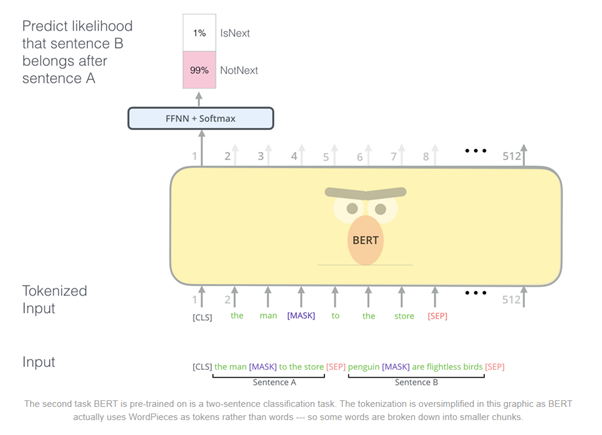
\includegraphics[width=10cm]{images/bert.png}
\caption{A representation of BERT}
\end{figure}

\section{Results}

\subsection{Simple RNN with ReLU on SNLI}

\textbf{Total Accuracy = 81.74 \%}\\
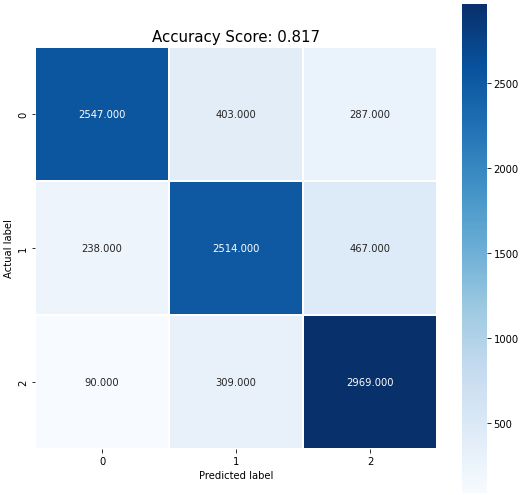
\includegraphics[width=7cm]{images/results/SNLIrelu.png}

\begin{table}[h]
\begin{tabular}{|l|l|l|l|}
\hline
  & \textbf{Precision} & \textbf{Recall} & \textbf{F1 Score} \\ \hline
\textbf{Entailment} & 0.89               & 0.79            & 0.83              \\ \hline
\textbf{Contradiction} & 0.78               & 0.78            & 0.78              \\ \hline
\textbf{Neutral} & 0.80               & 0.88            & 0.84              \\ \hline
\end{tabular}
\end{table}

\subsection{Simple RNN with ReLU on MultiNLI}

\textbf{Total Accuracy = 68.28 \%}\\
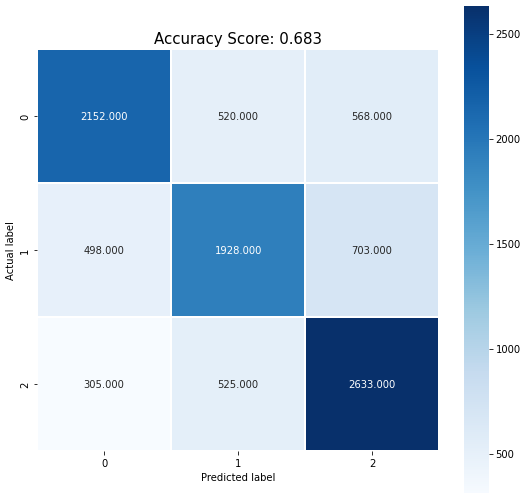
\includegraphics[width=7cm]{images/results/MNLIrelu.png}

\begin{table}[]
\begin{tabular}{|l|l|l|l|}
\hline
                       & \textbf{Precision} & \textbf{Recall} & \textbf{F1 Score} \\ \hline
\textbf{Entailment}    & 0.73               & 0.66            & 0.69              \\ \hline
\textbf{Contradiction} & 0.65               & 0.62            & 0.63              \\ \hline
\textbf{Neutral}       & 0.67               & 0.76            & 0.71              \\ \hline
\end{tabular}
\end{table}

\subsection{Simple RNN with Sigmoid on SNLI}
\textbf{Total Accuracy = 81.65 \%}\\
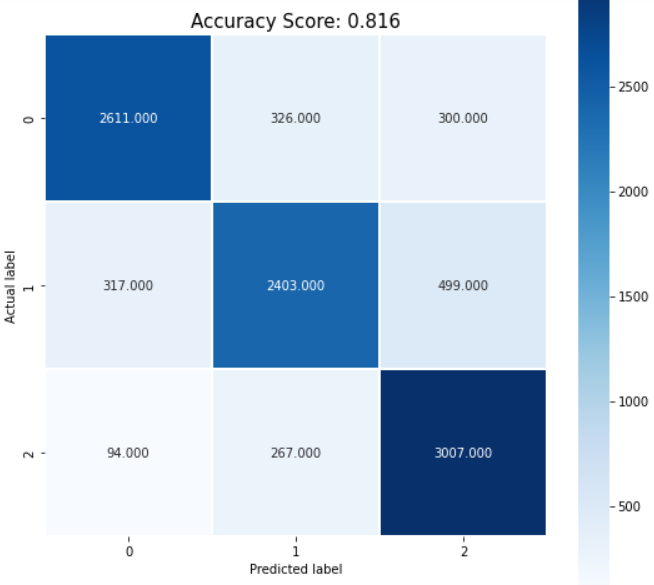
\includegraphics[width=7cm]{images/results/SNLIsigmoid.png}

\begin{table}[h]
\begin{tabular}{|l|l|l|l|}
\hline
                       & \textbf{Precision} & \textbf{Recall} & \textbf{F1 Score} \\ \hline
\textbf{Entailment}    & 0.86               & 0.81            & 0.83              \\ \hline
\textbf{Contradiction} & 0.80               & 0.75            & 0.77              \\ \hline
\textbf{Neutral}       & 0.79               & 0.89            & 0.84              \\ \hline
\end{tabular}
\end{table}

\subsection{Simple RNN with Sigmoid on MultiNLI}
\textbf{Total Accuracy = 67.84 \%}\\
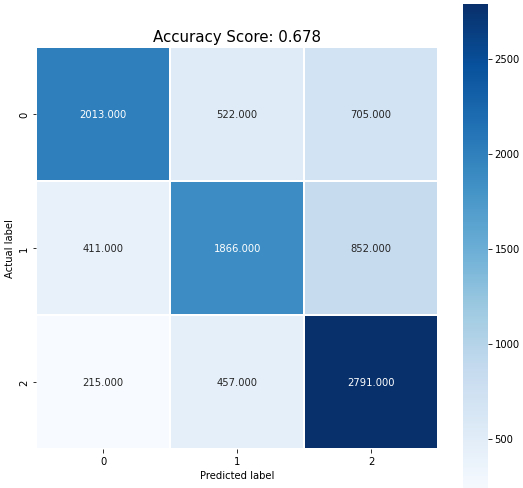
\includegraphics[width=7cm]{images/results/MNLIsigmoid.png}

\begin{table}[h]
\begin{tabular}{|l|l|l|l|}
\hline
                       & \textbf{Precision} & \textbf{Recall} & \textbf{F1 Score} \\ \hline
\textbf{Entailment}    & 0.76               & 0.62            & 0.68              \\ \hline
\textbf{Contradiction} & 0.66               & 0.60            & 0.62              \\ \hline
\textbf{Neutral}       & 0.64               & 0.81            & 0.71              \\ \hline
\end{tabular}
\end{table}

\subsection{Simple RNN with Softmax on SNLI}
\textbf{Total Accuracy = 79.69 \%}\\
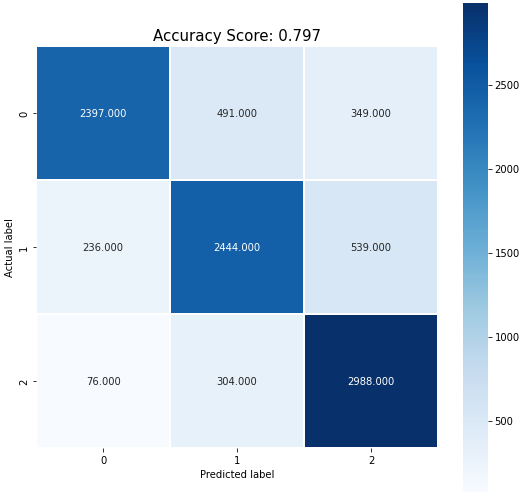
\includegraphics[width=7cm]{images/results/SNLIsoft.png}

\begin{table}[h]
\begin{tabular}{|l|l|l|l|}
\hline
                       & \textbf{Precision} & \textbf{Recall} & \textbf{F1 Score} \\ \hline
\textbf{Entailment}    & 0.88               & 0.74            & 0.81              \\ \hline
\textbf{Contradiction} & 0.75               & 0.76            & 0.76              \\ \hline
\textbf{Neutral}       & 0.77               & 0.89            & 0.82              \\ \hline
\end{tabular}
\end{table}

\subsection{Simple RNN with Softmax on MultiNLI}
\textbf{Total Accuracy = 67.10 \%}\\
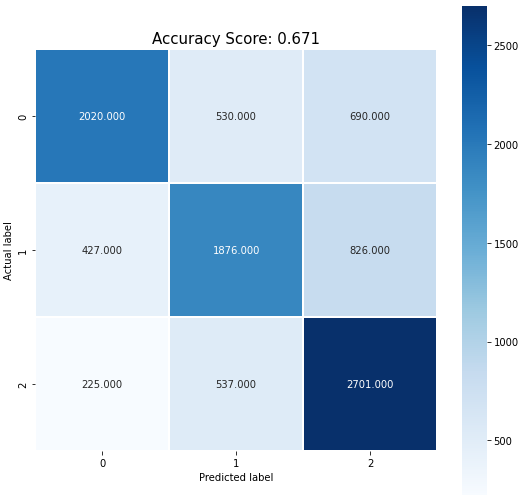
\includegraphics[width=7cm]{images/results/MNLIsoft.png}

\begin{table}[h]
\begin{tabular}{|l|l|l|l|}
\hline
                       & \textbf{Precision} & \textbf{Recall} & \textbf{F1 Score} \\ \hline
\textbf{Entailment}    & 0.76               & 0.62            & 0.68              \\ \hline
\textbf{Contradiction} & 0.64               & 0.60            & 0.62              \\ \hline
\textbf{Neutral}       & 0.64               & 0.78            & 0.70              \\ \hline
\end{tabular}
\end{table}

\subsection{LSTM on SNLI}
\textbf{Total Accuracy = 81.52 \%}\\
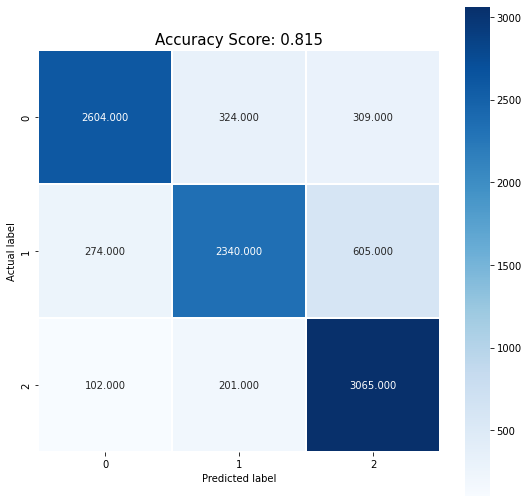
\includegraphics[width=7cm]{images/results/SNLIlstm.png}

\begin{table}[h]
\begin{tabular}{|l|l|l|l|}
\hline
                       & \textbf{Precision} & \textbf{Recall} & \textbf{F1 Score} \\ \hline
\textbf{Entailment}    & 0.87               & 0.80            & 0.84              \\ \hline
\textbf{Contradiction} & 0.82               & 0.73            & 0.77              \\ \hline
\textbf{Neutral}       & 0.77               & 0.91            & 0.83              \\ \hline
\end{tabular}
\end{table}

\subsection{GRU on SNLI}
\textbf{Total Accuracy = 82.84 \%}\\
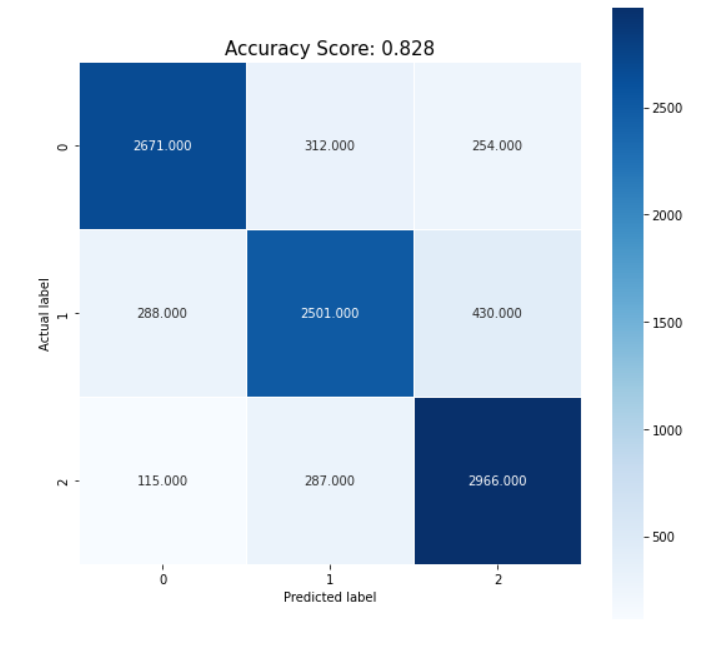
\includegraphics[width=7cm]{images/results/SNLIgru.png}

\begin{table}[h]
\begin{tabular}{|l|l|l|l|}
\hline
                       & \textbf{Precision} & \textbf{Recall} & \textbf{F1 Score} \\ \hline
\textbf{Entailment}    & 0.87               & 0.80            & 0.85              \\ \hline
\textbf{Contradiction} & 0.82               & 0.78            & 0.79              \\ \hline
\textbf{Neutral}       & 0.81               & 0.88            & 0.85              \\ \hline
\end{tabular}
\end{table}

\subsection{BERT on SNLI}
\textbf{Total Accuracy = 81.30 \%}\\
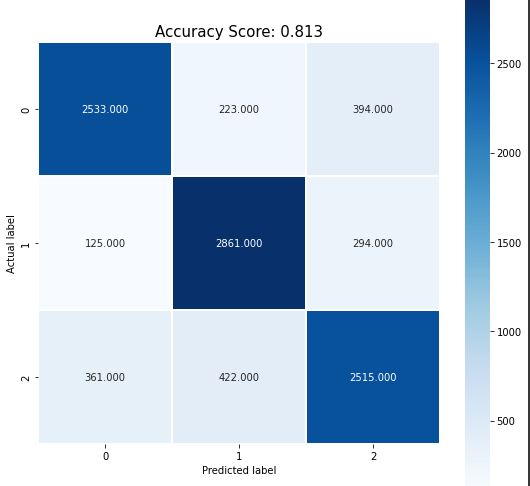
\includegraphics[width=7cm]{images/results/SNLIbert.png}

\begin{table}[h]
\begin{tabular}{|l|l|l|l|}
\hline
                       & \textbf{Precision} & \textbf{Recall} & \textbf{F1 Score} \\ \hline
\textbf{Entailment}    & 0.84               & 0.80            & 0.82              \\ \hline
\textbf{Contradiction} & 0.82               & 0.87            & 0.84              \\ \hline
\textbf{Neutral}       & 0.79               & 0.76            & 0.77              \\ \hline
\end{tabular}
\end{table}


\section{Observations}
\begin{itemize}
    \item{Analysing our more complex models, like the LSTM, GRU and BERT models, it is surprising to see that the more simplistic models based on the Simple RNN perform somewhat competitively.}
    \item{The larger, more complex models hence provide a lower performance-to-cost ratio when taking into account the memory and time needed to train these models.}
    \item{Our more complex models were never tested on the MultiNLI dataset. So instead, to compare the results of the simpler models with state-of-the-art Bi-directional LSTM models we referred to this \cite{b5} paper. The authors were able to achieve an accuracy of 72.1\% on a mismatched dataset which is the test dataset in our case for MultiNLI. As we saw before we were able to achieve 68.28\% which is not far off from the state-of-the-art Bi-directional LSTM model.}
    \item{Having seen leaderboards for NLI tasks, it is a trend that improvements tend to be minute and incremental. Hence our contribution, although modest, is a step forward.}
    \item{The trend among our models seems to be that entailment and neutral pairs are detected well, whereas the contradicting pairs are not detected so well. An outlier in this trend is the BERT model which, despite falling short in terms of overall accuracy, outperforms every other model in detecting contradicting statements which we see by the huge margin in f1 scores.}
\end{itemize}





\section*{Acknowledgments}
\begin{itemize}
    \item{Laughsinthestocks for the plots of the activation functions.}
    \item{Christopher Olah's \href{https://colah.github.io/posts/2015-08-Understanding-LSTMs/}{blog} for the LSTM diagram.}
    \item{Alammar, J (2018) in The Illustrated Transformer[\href{https://jalammar.github.io/illustrated-transformer/}{Blog post}] for the BERT diagram.}
\end{itemize}

\begin{thebibliography}{00}

\bibitem{b1} Samuel R. Bowman, Gabor Angeli, Christopher Potts, Christopher D. Manning. A large annotated corpus for learning natural language inference. \href{https://arxiv.org/abs/1508.05326}{	arXiv:1508.05326}
\bibitem{b2} Alexey Romanov, Chaitanya Shivade. Lessons from Natural Language Inference. \href{https://arxiv.org/abs/1808.06752}{arXiv:1808.06752}
\bibitem{b3} Adina Williams, Nikita Nangia, Sam Bowman. A Broad-Coverage Challenge Corpus for Sentence Understanding through Inference. Courant Institute of Mathematical Sciences. \href{https://aclanthology.org/N18-1101}{Association for Computational Linguistics, 2018}
\bibitem{b4} Jeffrey Pennington and Richard Socher and Christopher D. Manning. GloVe: Global Vectors for Word Representation. \href{http://www.aclweb.org/anthology/D14-1162}{Empirical Methods in Natural Language Processing (EMNLP), 2014}
\bibitem{b5} Alex Wang, Amanpreet Singh, Julian Michael, Felix Hill, Omer Levy, Samuel R. Bowman. \href{https://arxiv.org/abs/1804.07461}{arXiv:1804.07461}
\end{thebibliography}


\end{document}